\section*{Zielsetzung}
\label{sec:zielsetzung}

In diesem Versuch werden verschiedene Kennziffern sowie die Charakteristik eines Geiger-Müller-Zählrohres
bestimmt.

\section{Theorie}
\label{sec:Theorie}

\subsection{Aufbau und Funktionsweise}
\label{sec:aufbau}

Der Aufbau des Geiger-Müller-Zählrohres ist in \autoref{fig:querschnitt} dargestellt. Es besteht aus
einem Kathodenzylinder (Radius $R_\text{k}$) und einem mittig liegenden, axial verlaufenden
Anodendraht (Radius $R_\text{a}$) und wird mit einem Gasgemisch (z.B. Argon und verschiedene Alkohole) gefüllt.
\begin{figure}[H]
	\centering
	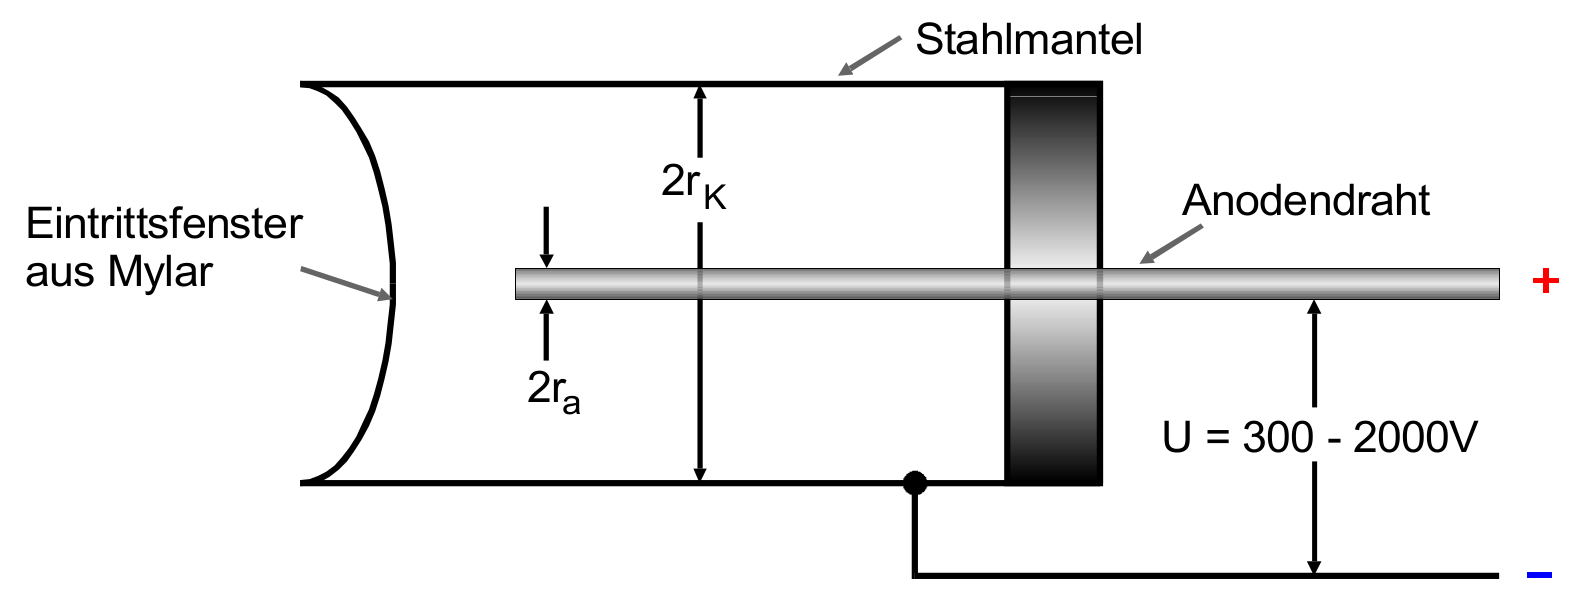
\includegraphics[width=0.8\textwidth]{content/querschnitt.png}
	\caption{Querschnitt durch ein Endfenster-Zählrohr \cite{sample}}
	\label{fig:querschnitt}
\end{figure}
\noindent
Bei Anlegen einer Spannung $U$ verhält sich das Rohr wie ein zylindrischer Kondensator, woraus die 
radialsymetrische elektrische Feldstärke
\begin{equation}
	E = \frac{U}{r \ln(r_\text{k} / r_\text{a})}
	\label{eqn:elektrisches-feld}
\end{equation}
folgt.
\\
Eine technische Schwierigkeit ist die Realisierung, dass $\alpha$- und
$\beta$-Teilchen in das Rohr eintreten, da diese sehr leicht mit ihrer Umgebung (also auch mit dem Stahlmantel)
wechselwirken. Dabei wurde in diesem
Versuch ein Endfensterzählrohr verwendet. Das bedeutet, dass eine Seite (in \autoref{fig:querschnitt} die linke
Seite) des Zählrohres aus einem dünnwandigen Material mit Atomen niedriger Ordnungszahl besteht. Das
Endfenster besteht hier aus d\"unner Mylar-Folie.
Aufgrund ihrer geringen Dichte k\"onnen selbst $\alpha$-Teilchen
in das Z\"ahlrohr eintreten.

\subsection{Spannungsbereiche}
\label{sec:spannungsbereiche}

Es soll jetzt ein geladenes Teilchen, welches in das Zählrohrvolumen eindringt, betrachtet werden. Unter
der Annahme, dass es vollständig absorbiert wird, wird es sich durch den Gasraum bewegen, bis es seine 
Energie durch Ionisationen abgegeben hat. Dabei wird im Mittel eine Energie von $26\ \si{\eV}$ 
abgegeben \cite{detektoren}.
Die Teilchen, die hier betrachtet werden, haben eine Energie in der Größenordnung $10^5\ \si{\eV}$, d.h. 
dass die Anzahl an Ionisation und der dabei freigesetzten Elektronen proportional zur Energie des 
einfallenden Teilchens sind.

\noindent
Dabei ist wichtig, dass die Vorgänge nach der ersten Ionisation im Zählrohr stark von der Spannung $U$ 
abhängen, der Zusammenhang ist in \autoref{fig:ionisationen-u} dargestellt.
\begin{figure}[H]
	\centering
	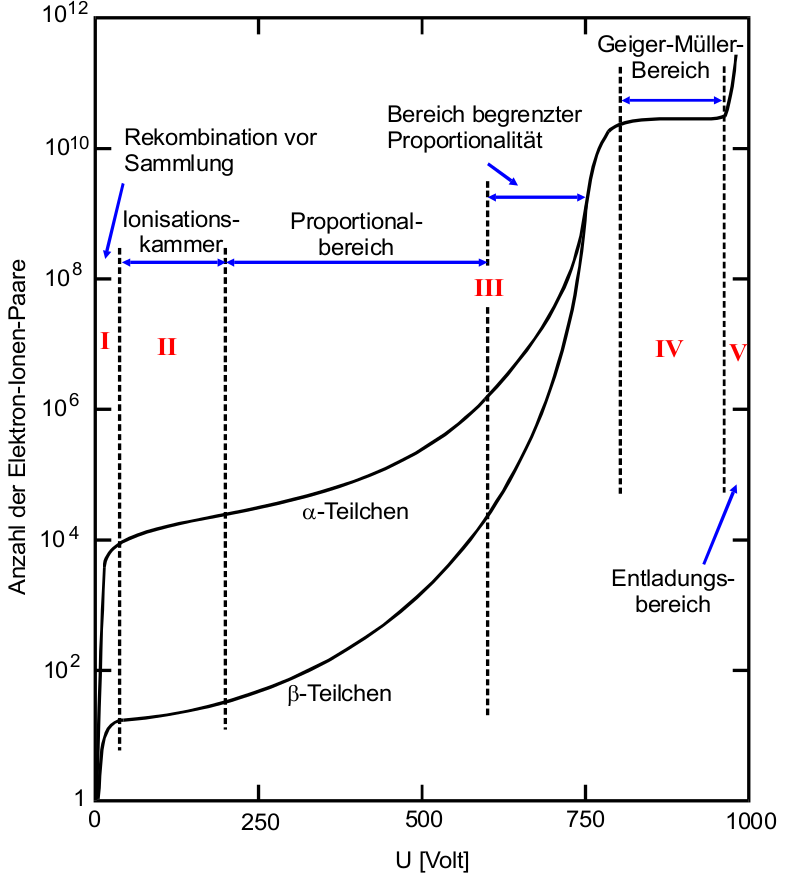
\includegraphics[width=0.6\textwidth]{content/ionisationen-u.png}
	\caption{Anzahl der erzeugten Elektron-Ionenpaare als Funktion der Spannung U bei einem
	Proportionalzählrohr (nach Kleinknecht, Detektoren für Teilchenstrahlen) \cite{sample}}
	\label{fig:ionisationen-u}
\end{figure}
Dabei sind einige Bereiche bei $U$ zu unterscheiden:
\begin{itemize}
	\item Für kleine Spannungen geht nur ein Teil der Ionisationselektronen zur Anode, der Rest geht 
		durch Rekombination verloren. (Entspricht Bereich \Romannum{1} in \autoref{fig:ionisationen-u})
	\item Bei höheren Spannungen (Bereich \Romannum{2} in \autoref{fig:ionisationen-u})
		sinkt die Rekombinationswahrscheinlichkeit ab, sodass die meisten erzeugten Elektronen
		die Anode erreichen. Der Ionisationsstrom ist dabei proportional der Intensität und Energie
		der einfallenden Strahlung. Unter diesen Vorraussetzungen wird ein Gerät als Ionisationskammer
		bezeichnet, eignet sich jedoch nur bei hohen Strahlungsintensitäten.
	\item Wird die Spannung noch weiter erhöht, erhalten die entstehenden Elektronen aufgrund der hohen Feldstärke
		genug Energie um weitere Ionisationen durchzuführen (sog. Stoßionisationen). Da auch die bei den
		Stoßionisationen entstehenden Elektronen weitere Ionisationen durchführen können, kann eine ganze
		Kaskade entstehen, die auch als Townsend-Lawine bezeichnet wird.
		\\
		Durch diese Lawinen sammelt sich jetzt am Anodendraht eine Ladung $Q$, welche als Ladungsimpuls 
		gemessen werden kann, aber dennoch proportional zur ursprünglichen Energie des einfliegenden
		Teilchens ist. Wegen dieser Proportionalität wird ein Betrieb in Bereich \Romannum{3} in 
		\autoref{fig:ionisationen-u} als Proportionalzählrohr bezeichnet.
	\item Nach dem Proportionalbereich folgt der Auslösebereich (Bereich \Romannum{4} in
		\autoref{fig:ionisationen-u}). Hier entstehen bei der primären Elektronenlawine UV-Photonen, welche
		sich im gesamten Zählrohr ausbreiten können und im gesamten Volumen weitere Elektronenkaskaden auslösen.
		Die Ladung $Q$ hängt jetzt nicht mehr von der Teilchenenergie, dafür aber vom Zählrohrvolumen und der 
		Spanung $U$ ab.
		\\
		Daher kann keine Energiemessung mehr stattfinden, nur Intensitätsmessungen. Dafür ist $Q$ auch mit
		geringem elektronischen Aufwand messbar.
\end{itemize}



\subsection{Einfluss der positiven Ionen}
\label{sec:einfluss-ionen}
\subsubsection{Totzeit}
\label{sec:totzeit}
Bisher wurden hier nur die Elektronen behandelt, welche aufgrund ihrer geringen Masse relativ schnell zur Anode 
wandern. Anders sieht es mit den positiven Ionen aus, welche sich länger im Gasraum aufhalten. Vorübergehend bauen
diese Ionen eine radialsymmetrische, positive Ladungsdichte auf, welche die Feldstärke senkt. Daher kann für ein Zeit
$T$ (``Totzeit``) keine Stoßionisation stattfinden und ein eintreffendes Teilchen wird nicht registriert. Nach der 
Totzeit
entstehen wieder Ladungsimpulse $Q$, diese sind zunächst nicht so hoch wie vorher, da die elektrische Feldstärke immer
noch niedriger ist als in \autoref{eqn:elektrisches-feld}. Da sich das elektrische Feld ``erholen`` muss, nennt man
diesen Zeitraum auch ``Erholungszeit``. 
In \autoref{fig:totzeit} sind Tot- und Erholungszeit dargestellt, wobei letztere nur ungenau bestimmt werden kann.
\begin{figure}[H]
	\centering
	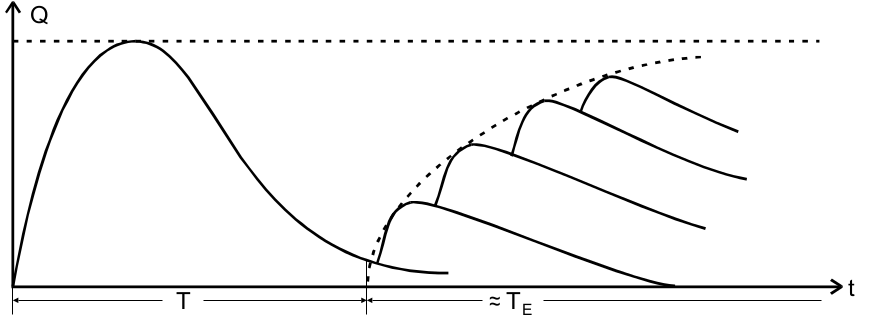
\includegraphics[width=0.8\textwidth]{content/totzeit.png}
	\caption{Tot- und Erholungszeit eines Zählrohres im Ladungs-Zeit-Diagramm \cite{sample}}
	\label{fig:totzeit}
\end{figure}

\subsubsection{Nachentladung}
\label{sec:nachentladung}

Ein weiterer Effekt tritt auf, wenn die positiven Ionen auf den Zählrohrmantel treffen. Bei ihrer Neutralisation wird
eine Energie freigesetzt, die größer als die Austrittsarbeit für die Elektronen ist, weswegen letztere in das Zählrohr
ausgeworfen werden können. Diese sog. ``Sekundärelektronen`` können im Zählrohr dann neue Entladungen zünden und 
 weitere Ladungsimpulse an der Anode auslösen, sog. Nachentladungen. Diese Nachentladungen finden (weil die
Ionen zuvor schon abgewandert sind) nach der Totzeit statt, weshalb sie das Eintreffen eines weiteren Teilchens 
vortäuschen.
\\
Offensichtlich sind die Nachentladungen unerwünscht, da sie die Präzision des Rohres stark in eine Richtung verringern.
Die Unterbindung der Nachentladungen geschieht durch die in \autoref{sec:aufbau} erwähnten Alkoholdämpfe im 
Zählrohr. Die Alkoholmoleküle besitzen eine geringere Ionisationsenergie als Argon, weswegen diese von den Ionen als 
Reaktionspartner bevorzugt werden. Sie verbrauchen die Energie 
jedoch bei Schwingungen innerhalb der großen Moleküle und können somit keine Sekundärelektronen erzeugen, wenn sie 
auf die Kathode treffen.

\subsection{Charakteristik des Zählrohres}
\label{sec:theo:charakteristik}

Ein Merkmal eines Zählrohres ist die Charakteristik. Dabei wird das Rohr mit konstanter Intensität bestrahlt und
die Spannung $U$ wird variiert. Der Graph $N(U)$ ($N$ sei nun die Anzahl an Ladungsimpulsen pro Zeiteinheit) ist dann
die Charakteristik des Zählrohres. In
\autoref{fig:theo:charakteristik} ist ein Beispiel für eine Charakteristik.
\begin{figure}[H]
	\centering
	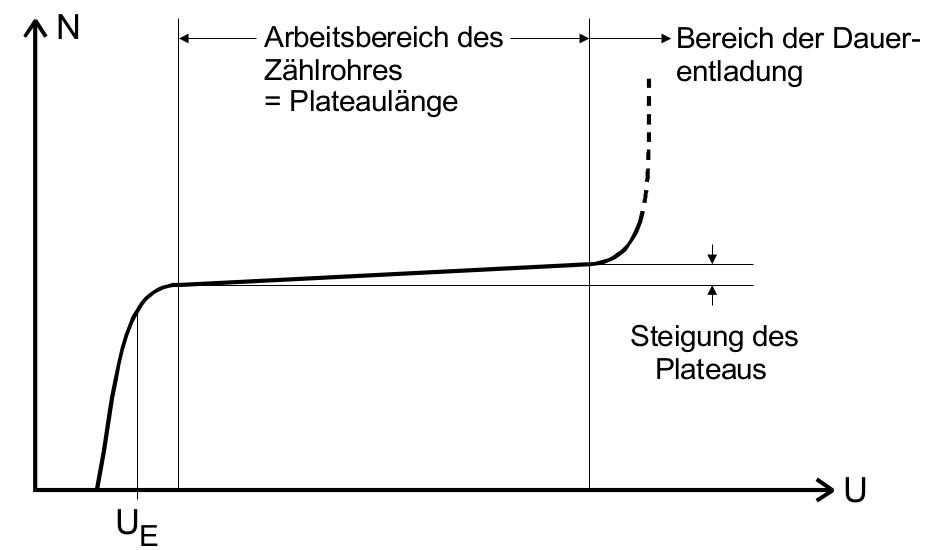
\includegraphics[width=0.6\textwidth]{content/charakteristik.png}
	\caption{Zählrohrcharakteristik (gemessene Ladungsimpulse bei konstanter Strahlungsintensität). $U_\text{E}$
	markiert den Start des Auslösebereichs. \cite{sample}}
	\label{fig:theo:charakteristik}
\end{figure}

\noindent
Auffällig ist dabei der flache, lineare Teil der Kurve, das Plateau. Bei einem idealen Zählrohr wäre die Steigung
im Plateau gleich null, in der Praxis wird aufgrund von Nachentladungen immer eine leichte Steigung entstehen. 
Allgemein gilt
jedoch, dass ein flacheres und längeres Plateu für eine höhere Qualität des Zählrohres spricht.
\\
Auffällig ist auch die starke Steigung rechts vom Plateau. Dies ist die Folge von Selbstentladungen aufgrund 
der hohen Feldstärke. Dort sorgt dann ein eintreffendes Teilchen für eine Dauerentladung. Wegen den hohen Stromdichten
wird das Zählrohr in diesem Bereich schnell zerstört.

\subsection{Ansprechvermögen des Zählrohres}
\label{sec:theo:ansprechvermoegen}

Das Ansprechverm\"ogen steht f\"ur die Wahrscheinlichkeit, dass ein einfallendes Teilchen tats\"achlich als solches detektiert wird.
Da $\alpha$- und $\beta$-Teilchen ein hohes Ionisationsvermögen besitzen, liegt das Ansprechvermögen
bei nahezu $100\%$. Mit der anfangs erwähnten Mylar-Folie (vgl. \autoref{sec:aufbau}) ist auch das Eindringen in
den Zählraum realisiert.
\\
Im Vergleich zu den geladenen Teilchen ist das Ansprechvermögen von Photonen jedoch sehr niedrig. Bei hochenergetischen
Photonen (z.B. $\gamma$-Strahlung) liegt es bei ungefähr $1\%$, weshalb nur $\gamma$-Strahlung mit hohen
Intensitäten gemessen werden kann.
\\
Mit einem schweren Füllgas (z.B. Xenon) können allerdings die niederenergetischen Röntgen-Quanten gut gemessen werden.

\subsection{Bestimmung der Totzeit}
\label{sec:bestimmung-totzeit}

Für die Bestimmung der Totzeit (vgl. \autoref{sec:totzeit}) stehen zwei Methoden zur Verfügung:
\begin{enumerate}
	\item Oszillographische Messung
	\item Zwei-Quellen-Methode
\end{enumerate}
Im Folgenden werden beide Messmethoden erläutert.

\subsubsection{Oszillographische Messung der Totzeit}
\label{sec:theo:oszillographisch}

Es wird eine hohe Strahlungsintensität eingestellt, zusätzlich muss der Trigger des Oszillographen auf die 
Anstiegsflanke gestellt werden. Dadurch wird ein Oszillogramm ähnlich zu dem in \autoref{fig:totzeit} erzeugt.
\\
Bei hoher Intensität, so die Theorie, folgt ein Puls auf den Anderen direkt nach der Totzeit, weswegen hier die Zeit zwischen zwei Pulsen als Totzeit angenommen werden kann.z
Bei hoher Intensität, so die Theorie, folgt ein Puls auf den Anderen direkt nach der Totzeit, weswegen wir hier die
Zeit zwischen zwei Pulsen als Totzeit annehmen können.

\subsubsection{Zwei-Quellen-Methode}
\label{sec:theo:zwei-quellen}

Wie in \autoref{sec:totzeit} erklärt, ist aufgrund der Totzeit $T$ die Impulsrate der detektierten Teilchen $N_\text{r}$
immer kleiner als die Rate der eindringenden Teilchen $N_\text{w}$. So ist bei einer Impulsrate $N_\text{r}$ das 
Messrohr für die Zeit $TN_\text{r}$ unempfindlich. Wird über einen Zeitraum $t$ gemessen, so ist die Zeit wo
das Messrohr tatsächlich empfindlich war $(1-TN_\text{r})t$. Die wahre Impulsrate ist daher
\begin{equation}
	N_\text{w} = \frac{\text{Gemessene Impulse}}{\text{Tatsächliche Messzeit}}
	= \frac{N_\text{r} t}{(1-TN_\text{r}) t} = \frac{N_\text{r}}{1 - TN_\text{r}}.
	\label{eqn:wahre-zaehlrate}
\end{equation}
\noindent
Auf Grundlage von \autoref{eqn:wahre-zaehlrate} beruht die Zwei-Quellen-Methode, bei der, wie der Name andeutet, mit
zwei radioaktiven Quellen gearbeitet wird.
Zunächst wird die Zählrate $N_1$, die das Präparat 1 im Zählrohr hervorruft, gemessen. 
Dann wird das 2. Pr\"aparat hinzugef\"ugt und es wird die gemeinsame Z\"ahlrate $N_{1+2}$ gemessen, wobei dadrauf geachtet werden muss, Quelle 1 nicht zu verschieben. 
Zuletzt wird Präparat 1 entfernt und die Zählrate $N_2$ des zweiten Präparats gemessen.
\\
Hätte das Zählrohr keine Totzeit würden sich die Impulse addieren, also müsste der Zusammenhang
\begin{equation}
	N_{1+2} = N_1 + N_2
\end{equation}
gelten. \\
In der Praxis gilt jedoch
\begin{equation}
	N_{1+2} < N_1 + N_2.
\end{equation}
Gemäß \autoref{eqn:wahre-zaehlrate} dringen während der Messung
\begin{equation}
	N_{{\text{w}_i}} = \frac{N_i}{1 - TN_i} 
		\quad \text{für } i \in \{1, 2, 1+2\}
\end{equation}
Teilchen ins Zählrohr ein.
\\
Hierbei gilt $N_{\text{w}_{1+2}} = N_{\text{w}_{1}} + N_{\text{w}_{2}}$, damit folgt
\begin{equation}
	\frac{N_{1+2}}{1 - TN_{1+2}} =
	\frac{N_1}{1 - TN_1} +
	\frac{N_2}{1 - TN_2} .
	\label{eqn:theo:paar-brueche}
\end{equation}
\noindent
Die Größen $N_1$, $N_2$ und $N_{1+2}$ werden gemessen, daher kann mit \autoref{eqn:theo:paar-brueche} die 
Totzeit bestimmt werden. Für $T^2N_i^2 \ll 1$ mit $i \in \{1, 2, 1+2\}$ gilt dann näherungsweise
\begin{equation}
	T \approx \frac{N_1 + N_2 - N_{1+2}}{2N_1N_2}.
	\label{eqn:totzeit-naeherung}
\end{equation}

\subsection{Messung der pro Teilchen freigesetzten Ladungsmenge}
\label{sec:theo:messung-freigesetzte-ladungsmenge}

Mit einem Strommessgerät zwischen Anode und Kathode (vgl. \autoref{fig:aufbau}) kann der zeitlich gemittelte
Zählrohrstrom
\begin{equation}
	\overline{\mathbf{I}} = \frac 1 \tau \int_0^\tau \frac{U(t)}{R} dt
	\label{eqn:theo:mittlerer-zaehlrohrstrom}
\end{equation}
gemessen werden.
\\
Wenn in einem Zeitintervall $\Delta t$ $Z$ Teilchen detektiert wurden und ein Teilchen den Transport von der Ladung
$\Delta Q$ veranlasst, so gilt die Gleichung
\begin{equation}
	\overline{\mathbf{I}} = \frac{\Delta Q}{\Delta t} Z.
\end{equation}